\documentclass[letterpaper,11pt]{article}

\author{Jacob Thomas Errington}
\date{21 February 2017}
\title{Assignment \#3\\Formal verification -- COMP 525}

\usepackage[margin=2.0cm]{geometry}
\usepackage{amsmath,amssymb,amsthm}
\usepackage{tikz}
\usetikzlibrary{automata, graphs, arrows}

\newtheorem{prop}{Proposition}

\renewcommand{\thesection}{Question \arabic{section}}
\newcommand{\question}{\section}
\renewcommand{\complement}{\overline}
\newcommand{\eventually}{\lozenge}
\newcommand{\always}{\square}
\newcommand{\nmodels}{\nvDash}
\newcommand{\step}{\bigcirc}
\DeclareMathOperator{\untilOp}{\mathtt{U}}
\newcommand{\until}{\untilOp{}}
\newcommand{\Land}{\bigwedge}
\newcommand{\parens}[1]{\left(#1\right)}

\newcommand{\enumalpha}{\renewcommand\labelenumi{(\alph{enumi})}}
\newcommand{\quadequiv}{\quad \equiv \quad}
\newcommand{\nquadequiv}{\quad \not \equiv \quad}
\DeclareMathOperator{\Sat}{Sat}
\newcommand{\sat}[1]{\Sat{\parens{#1}}}
\DeclareMathOperator{\Odd}{odd}
\newcommand{\odd}[1]{\Odd{\parens{#1}}}

\begin{document}

\maketitle

\question{Writing $\omega$-regular expressions for B\"uchi automata}

The left automaton can be represented by
\begin{equation*}
    (A \Sigma^* A + C \Sigma^* C)^\omega
\end{equation*}

The right automaton can be represented by
\begin{equation*}
    (B + C)^* (A (BC)^* ( (BC)^\omega + BA^\omega ) + B A^\omega )
\end{equation*}

\question{Properties of DBAs}

\begin{prop}
    The class of DBAs is not closed under complementation.
\end{prop}

\begin{proof}
    To see this, we will find a DBA whose complement language cannot be
    recognized by a DBA. We know that the language represented by the
    $\omega$-regular expression $R = (A + B)^* B^\omega$ cannot be recognized
    by a DBA. Let $L(R)$ be the language recognized by an NBA represented by
    the expression $R$. In natural language, this language is the set of all
    strings with only finitely many $A$. Hence, if a string is \emph{not} in
    this language, then it has infinitely many $A$. Consequently, the
    complement language, in which $A$ appears infinitely many times,
    $\complement{L(R)}$ is recognized by an NBA represented by the
    $\omega$-regular expression $\complement{R} = (\Sigma^* A)^\omega$.

    We claim that there is a DBA represented by $\complement{R}$. Figure
    \ref{fig:dba} shows a deterministic automaton to recognize the language of
    the expression $\complement{R}$.

    However, $\complement{\complement{R}} = R$ is known to not be recognizable
    by a DBA. Hence, DBAs are not closed under complementation.

    \begin{figure}[ht]
        \begin{center}
            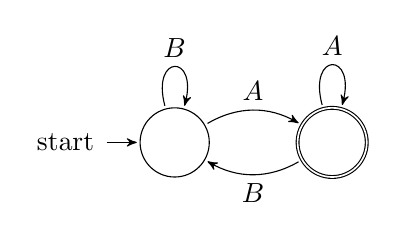
\begin{tikzpicture}[
                    node distance=2cm,
                    auto,
                    >=stealth',
                    shorten <=1pt,
                    shorten >=1pt,
                ]
                \node[state,initial] (s) {} ;
                \node[state,accepting,right of=s] (t) {} ;

                \graph[use existing nodes]{
                    s ->[loop above,edge label=$B$]
                    s ->[edge label=$A$,bend left=30]
                    t ->[loop above,edge label=$A$]
                    t ->[edge label=$B$,bend left=30]
                    s ;
                } ;
            \end{tikzpicture}
        \end{center}
        \caption{
            A DBA for the language of the expression $\complement{R}$.
        }
        \label{fig:dba}
    \end{figure}
\end{proof}

\question{Satisfying LTL formulas}

\begin{enumerate}
    \item $TS \nmodels \eventually \always c$

        Since after either start state, we reach infinite alternation between
        $s_4$ and one of $s_3, s_5, s_2$. In $s_4$, $c$ is false, whereas in
        each of $s_3, s_5, s_2$, $c$ is true. The infinite portion of any run
        through this automaton will have a strict alternation of $c$ being true
        and false. Consequently, we cannot have $\always c$ no matter how long
        we wait.

    \item $TS \models \always \eventually c$

        By the same argument about the infinite portion of the runs, $c$ occurs
        infinitely often.

    \item $TS \models \step \neg c \implies \step \step c$

        This deals just with the beginning of the string, and doesn't make any
        ``infinite claims''.
        This means we can exhaustively check the prefixes of relevant lengths.
        In particular, we have $\sigma_1 = s_1 s_3 s_4 \tau$,
        $\sigma_2 = s_1 s_4 \tau$, and $\sigma_3 = s_2 s_4 \tau$. Notice that
        in the first letter in $\tau$, $c$ is true (these are the states
        reachable in one step from $s_4$).

        $\sigma_1$ satisfies the property, since the premise of the implication
        is not satisfied, and from falsehood follows anything.
        $\sigma_2$ satisfies the property, since the premise is satisfied, and
        the first state in $\tau$ has $c$ true.
        $\sigma_3$ satisfies the property for the same reason.

    \item $TS \nmodels \always a$

        Any run starting in $s_2$ starts with $\neg a$, so those runs don't
        satisfy the property.

    \item $TS \models a \until \always (b \lor c)$

        In runs starting from $s_1$, we have $a$ true, and anywhere we go from
        there, we always have $b \lor c$ true.

        In runs starting from $s_2$, we don't have $a$. However, we have
        $b \lor c$ true right away. This is fine, because ``until'' allows the
        left hand side to possibly occur zero times.

    \item $TS \nmodels (\step \step b) \until (b \lor c)$

        Consider the run $\sigma = s_1 s_4 s_2 s_4 \tau$. It does reach a state
        where $b \lor c$ is true (namely $s_4$ right at the second letter), but
        it does not satisfy $\step \step b$ for all states leading up to that
        point. In particular, $\step \step b$ is not true of the initial state
        in this run.
\end{enumerate}

\question{Elevator system}

To each floor $i$, we assign the following atomic propositions.
\begin{itemize}
    \item $r_i$ -- the call button is active on floor $i$
    \item $d_i$ -- the door is open on floor $i$
    \item $e_i$ -- the elevator is serving floor $i$
\end{itemize}

Here are translations of some properties into LTL formulas.

\begin{enumerate}
    \item ``The doors are safe.''

        \begin{equation*}
            \always\parens{\Land_i \parens{d_i \implies e_i}}
        \end{equation*}

    \item ``A requested floor will be served sometime.''

        \begin{equation*}
            \always\parens{
                \Land_i \parens{
                    c_i \implies \eventually e_i
                }
            }
        \end{equation*}

    \item ``Again and again, the evelator returns to floor 0.''

        \begin{equation*}
            \always\parens{
                \neg e_0 \implies \eventually e_0
            }
        \end{equation*}

    \item ``When the top floor is requested, the elevator serves it immediately
        and does not stop on the way there.''

        \begin{equation*}
            \always\parens{
                r_3 \implies \parens{
                    \parens{
                        \Land_{i \neq 3} \neg e_i
                    }
                    \until
                    e_3
                }
            }
        \end{equation*}
\end{enumerate}

\question{Deciding equivalence of LTL formulas}

\begin{enumerate}
        \enumalpha
    \item
        $
        \always \varphi \implies \eventually \psi
        \quadequiv
        \varphi \until \parens{\psi \lor \neg \varphi}
        $

        \begin{proof}
            Suppose $\sigma$ satisfies LHS.
            \begin{description}
                \item[Case] $\always \varphi$ is true. Then, we have that
                    somewhere in $\sigma$, $\psi$ is true. Since $\varphi$ is
                    always true, it will in particular have been true up till
                    the point where $\psi$ is true. Hence, it satisfies RHS.
                \item[Case] $\neg \always \varphi$ is true. Let $i$ be the
                    least index such that $\sigma[i]$ does not have $\varphi$
                    true. Then, $\varphi$ must be true for all states leading
                    up to index $i$. Hence, $\sigma$ it satisfies RHS.
            \end{description}

            Suppose $\sigma$ satisfies RHS. Then, we have at some point $i$
            that $\psi \lor \neg \varphi$ is true.
            \begin{description}
                \item[Case] it's $\psi$ that becomes true at index $i$. Then we
                    have that leading up to this point, $\varphi$ is true. If
                    $\varphi$ continues to be true past this point, then we
                    will have $\always \varphi$ and $\eventually \psi$, so this
                    string satisfies LHS. If $\varphi$ stops being true at
                    some point, then the string will trivially satisfy LHS.

                \item[Case] it's $\neg \varphi$ that becomes true at index
                    $i$. Then we have $\neg \always \varphi$, so the string
                    trivially satisfies LHS.
            \end{description}
        \end{proof}

    \item
        $
        \eventually \always \varphi \implies \always \eventually \psi
        \quadequiv
        \always\parens{
            \varphi \until \parens{
                \psi \lor \neg \varphi
            }
        }
        $

        \begin{proof}
            Suppose $\sigma$ satisfies
            $\eventually \always \varphi \implies \always \eventually \psi$.
            \begin{description}
                \item[Case] $\eventually \always \varphi$ is true.
                    Then we have $\always \eventually \psi$. Pick an arbitrary
                    time $i$. At some point $j \geq i$ later, $\psi$ becomes
                    true (since it is true infinitely many times).  If
                    $\varphi$ is true everywhere from $i$ up to $j$, then the
                    string satisfies RHS as we have $\varphi \until (\psi \lor
                    \neg \varphi)$.  Else, there exists $k$ with $i \leq k < j$
                    such that at time $k$, we have that $\neg \varphi$ is true.
                    Take the least such $k$. Then from $i$ up to $k$, we have
                    that $\varphi$ is true, and at time $k$, $\neg \varphi$ is
                    true.  Hence we have that $\varphi \until (\psi \lor \neg
                    \varphi)$ holds.

                \item[Case] $\eventually \always \varphi$ is not true.
                    From $\neg \eventually \always \varphi$,
                    we infer that $\always \eventually \neg \varphi$.
                    Hence, $\neg \varphi$ occurs infinitely often.
                    Take an arbitrary time $i$. We need to show that at some
                    $j \geq i$, it holds that $\psi \lor \neg \varphi$ is true
                    and from $i$ up to $j$ that $\varphi$ is true.
                    We know there exists a $j \geq i$ such that $\neg \varphi$
                    is true, since $\neg \varphi$ occurs infinitely often. Take
                    the least such $j$. Then, up till $j$, $\varphi$ is true.
                    Hence we have at an arbitrary time that
                    $\varphi \until (\psi \lor \neg \varphi)$ is true, so
                    $\sigma$ satisfies RHS.
            \end{description}

            Next suppose $\sigma$ satisfies RHS, i.e. that at any time $i$,
            there is a later time $j \geq i$ such that $\psi \lor \neg \varphi$
            is true and until that point, $\varphi$ is true.
            Suppose that from some point $p$ onwards, $\varphi$ is always true.
            We need to show that $\psi$ occurs infinitely often.
            To do this, we will work exclusively in the time frame in which
            $\varphi$ is always true.
            Take an arbitrary time $i \geq p$. There exists a time $j \geq i$
            such that $\psi \lor \neg \varphi$ is true. Since $\varphi$ is
            always true beyond $p$, the right component of this disjunction is
            impossible. Hence at point $j$, $\psi$ is true.
            Since we showed that for any time $i$ beyond $p$, $\psi$ occurs
            later, we can inductively find infinitely many times where $\psi$
            occurs.
            For the base case, take $i_0 = p$ and apply the above argument to
            find $j_0$ where $\psi$ is true. Then take $i_1 = j_0 + 1$ and
            repeat to find $j_1$, and so on. Hence, $\psi$ occurs infinitely
            often.
        \end{proof}

        \setcounter{enumi}{3} % skip to problem d
    \item
        $
        \eventually \parens{\varphi \land \psi}
        \nquadequiv
        \eventually \varphi \land \eventually \psi
        $

        This is intuitively false because the LHS requires that both $\varphi$
        and $\psi$ be true \emph{in the same state} eventually. The RHS is
        weaker: $\varphi$ and $\psi$ can occur at different times.

        Figure \ref{fig:ts-counterexample-1} shows a transition system
        satisfying the RHS but not the LHS.

        \begin{figure}[ht]
            \centering
            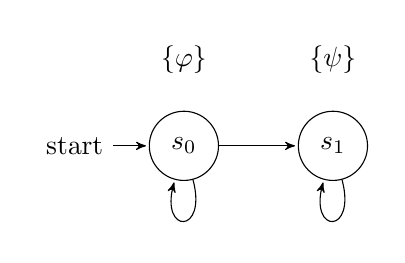
\begin{tikzpicture}[
                    ->,
                    >=stealth',
                    shorten >=1pt,
                ]
                \matrix[row sep=1em, column sep=1cm]{
                    \node (A') {$\{\varphi\}$} ;
                    &
                    \node (B') {$\{\psi\}$} ; \\

                    \node[initial,state] (A) {$s_0$} ;
                    &
                    \node[state] (B) {$s_1$} ; \\
                } ;

                \graph[use existing nodes]{
                    A ->[loop below] A -> B -> [loop below] B ;
                } ;
            \end{tikzpicture}
            \caption{
                A transition system satisfying
                $\eventually \varphi \land \eventually \psi$
                but not
                $\eventually \parens{\varphi \land \psi}$.
            }
            \label{fig:ts-counterexample-1}
        \end{figure}

        \setcounter{enumi}{6} % jump to problem g
    \item
        $
        \always \eventually \varphi \implies \always \eventually \psi
        \nquadequiv
        \always \parens{
            \varphi \implies \eventually \psi
        }
        $

        \begin{proof}
            This is easy to see. Suppose we have a string satisfying LHS, but
            in which $\varphi$ does not occur infinitely many times. Then we
            cannot infer that $\psi$ occurs infinitely many times, because the
            premise of the implication is not true; $\psi$ may not even ever be
            true! In particular, if that's the case, then it will not be true
            in such strings that whenever $\varphi$ is true that we can find a
            later time at which $\psi$ is true. Hence such strings, which
            satisfy the LHS, do not satisfy the RHS.
        \end{proof}

    \item
        $
        \parens{\varphi \until \psi} \until \psi
        \quadequiv
        \varphi \until \psi
        $

        \begin{proof}
            Suppose $\sigma$ satisfies LHS.
            Then at some time $i$, we have that $\psi$ is true, and up to that
            point, $\varphi \until \psi$ is true. Specifically, for all
            $j < i$, we can find $k \geq j$ such that $\psi$ is true and for
            all $l$ such that $j \geq l < k$, $\varphi$ is true.

            We want to show that there exists a time at which $\psi$ becomes
            true, and for all times before then, $\varphi$ is true.

            Let $i$ be the least time at which $\psi$ becomes true due to the
            outer until.
            If $i = 0$, then $\psi$ is immediately true. In that case the RHS
            is trivially satisfied by this string.
            Now suppose the least time $i$ at which $\psi$ becomes true is
            greater than zero.
            If $\varphi$ is true for all $l < i$, then the RHS is satisfied.
            Otherwise, let $j < i$ be the least time at which $\varphi$ becomes
            not true. Then, because of the inner until, we can find $k \geq j$
            such that $\psi$ is true at time $k$ and $\varphi$ is true at all
            times before $j$. But since $\varphi$ is not true at time $j$, $k$
            must be equal to $j$. But then we found a time at which $\psi$ is
            true and $\varphi$ is true leading up to that point, so the string
            satisfies the RHS as well.

            Next suppose $\sigma$ satisfies RHS.
            Then at some time $i$, $\psi$ is true, and at all times $j < i$,
            $\varphi$ is true.
            Pick an arbitrary time $j < i$. At this point $j$, we can find a
            later time at which $\psi$ is true, (namely at time $i$,) and until
            that point $\varphi$ is true, since at all $k < i$, $\varphi$ is
            true. Hence, $\sigma$ satisfies LHS.
        \end{proof}
\end{enumerate}

\question{Satisfaction of CTL formulas}

\begin{enumerate}
    \item $TS \models \forall (a \until b) \lor \exists \step (\forall \always b)$

        To see this, first look at $s_3$. Every string starting here trivially
        satisfies $a \until b$ since $b$ is true in the first state.
        Second, look at $s_0$. There exists a path such that if we take one
        step along it, we discover that $b$ is always true: this is the path
        that begins by transitioning to $s_4$. Hence, each initial state of
        $TS$ satisfies $\Phi_1$.

        \begin{equation*}
            \sat{\Phi_1} = \{ s_0, s_1, s_2, s_3, s_4 \}
        \end{equation*}

    \item $TS \nmodels \forall \always \forall (a \until b)$

        To see this, look at $s_3$. The path $\pi = s_3 s_0 s_4^\omega$
        is such that $\pi \nmodels \always \forall (a \until b)$. To see this,
        look at $s_0$. It is not that case that for any path starting here, we
        have $a \until b$. To see this, consider the path
        $\pi^\prime = s_0 s_4^\omega$. $b$ becomes true, yet $a$ is never true
        in this path.

        \begin{equation*}
            \sat{\Phi_2} = \{ s_4 \}
        \end{equation*}
\end{enumerate}

\question{Consequences of CTL state formula satisfaction}

\begin{enumerate}
    \item It is not the case that
        if $s \models \exists \always a$, then $s \models \forall \always a$.

        Figure \ref{fig:ts-counterexample-2} shows a transition system in which
        the premise is true but the consequence is not.

        \begin{figure}[ht]
            \centering
            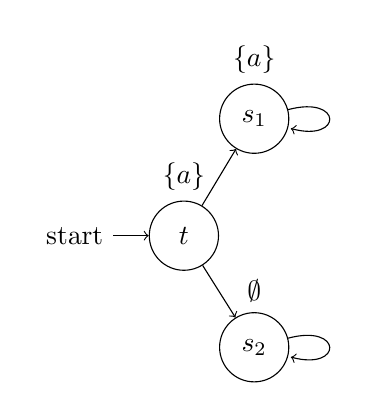
\begin{tikzpicture}
                \matrix{
                    & \node[label={$\{a\}$},state] (s1) {$s_1$} ; \\
                    \node[label={$\{a\}$},initial,state] (t) {$t$} ; & \\
                    & \node[label={$\emptyset$},state] (s2) {$s_2$} ; \\
                } ;
                \graph[use existing nodes]{
                    t -> {
                        s1 ->[loop right] s1,
                        s2 ->[loop right] s2
                    } ;
                } ;
            \end{tikzpicture}
            \caption{
                $s \models \exists \always a$, but
                $s \nmodels \forall \always a$.
            }
            \label{fig:ts-counterexample-2}
        \end{figure}

    \item If $s \models \forall \always a$, then $s \models \exists \always a$.

        \begin{proof}
            To see this, is suffices to notice two things.
            First, if we have a universally quantified statement over a
            nonempty domain, then we can choose an arbitrary element from that
            domain, and it will be a witness to the corresponding existential
            claim.
            Second, the domains we're dealing with in this scenario are always
            nonempty. Specifically, in every state, there is at least one
            transition leaving that state. This is because we're dealing with
            necessarily infinite strings; if there were a state with no arrows
            leaving it, then the string would \emph{end} at this state if ever
            it were reached.

            Hence, suppose we have a state $s$ such that
            $s \models \forall \always a$. Then just take an arbitrary path
            from this state, and it will be a witness of $\exists \always a$.
        \end{proof}
\end{enumerate}

\question{$\mu$-LTL}

\begin{enumerate}
    \item There is no problem at all, because the least fixed point operator
        $\mu$ is defined in terms of the greatest fixed point operator $\nu$.
        Observe the equivalence
        \begin{align*}
            \neg \always \neg \varphi
            = \neg \nu X . \neg \varphi \land \step X
            = \neg \nu X . \neg \varphi \land \neg \step \neg X
            = \neg \nu X . \neg (\varphi \lor \step \neg X)
            = \mu X . \varphi \lor \step X
        \end{align*}
        since $\mu X . \psi(X) \equiv \neg \nu X . \neg \psi (\neg X)$.

    \item $\nu X . p \land \step \step X$

    \item If we used the least fixed point operator $\mu$ instead, we would
        find that the empty set is a fixed point. To see this, we consider the
        Kleene fixed point theorem which gives an algorithm for computing the
        least fixed point by iterating the application of a monotone function
        to the least element of the lattice. The least element of the lattice
        in this case is $\emptyset$.
        The monotone function is $f(S) = p \land \step \step S$.
        But then, notice that $f(\emptyset) = \emptyset$, as there are no
        states such that taking two steps away we find that we are in no
        state!

    \item The formula
        $
        \phi =
        p
        \land
        \always (p \implies \step \neg p)
        \land
        \always (\neg p \implies \step p)
        $
        does not express $\odd{p}$ because it enforces a strict alternation.
        Whereas $\odd{p}$ should be satisfied by $p^\omega$, this string does
        not satisfy $\phi$.
\end{enumerate}

\end{document}
